\documentclass{beamer}

\usepackage[utf8]{inputenc}
\usepackage{caption}
\captionsetup[figure]{font=scriptsize,labelfont=scriptsize}
% \usepackage{utopia}
\usepackage{animate}
\usepackage{epigraph}

\setlength\epigraphwidth{8cm}
\setlength\epigraphrule{0pt}

\usetheme{Madrid}
\usecolortheme{seahorse}

\title[Deep Reinforcement Learning]{Deep Reinforcement Learning}
\subtitle{Scientific Initiation}
\author[Resck]{Lucas Emanuel Resck Domingues}
\institute[FGV]
{
  Escola de Matemática Aplicada \\
  Fundação Getulio Vargas
}
\date[2020]
{March 2020}

\AtBeginSection[]
{
  \begin{frame}
    \frametitle{Table of Contents}
    \tableofcontents[currentsection]
  \end{frame}
}

\setbeamertemplate{caption}[numbered]

\begin{document}

    \frame{\titlepage}

    \begin{frame}
        \frametitle{Table of Contents}
        \tableofcontents
    \end{frame}

    \section{Introduction}

        \begin{frame}
            \frametitle{Motivation}

            \begin{itemize}
                \item I wanted to do Scientific Initiation in Machine Learning;
                \item Reinforcement Learning is a quite promising area, because of the potential of applications;
                \item Deep Learning is one of the most powerful Machine Learning areas, because DNN can reach such degree of generalization;
                \item It seems that Deep Reinforcement Learning has very impressive powerful applications and it's on mainstream.
            \end{itemize}

        \end{frame}

        \begin{frame}
            \frametitle{Intuition}

            \begin{figure}
                \centering
                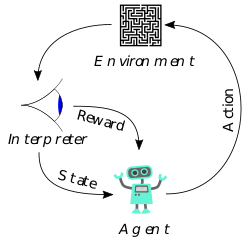
\includegraphics[width=0.6\textwidth]{figures/rl.png}
                \caption{Reinforcement Learning example (\href{https://en.wikipedia.org/wiki/Reinforcement_learning}{Wikipedia})}
                \label{fig14:rl}
            \end{figure}

        \end{frame}

    % \section{Imitation Learning}

    %     \begin{frame}
    %         \frametitle{Terminology}
    %         At time $t$:
    %         \begin{itemize}
    %             \item $s_t$: the state of the enviroment;
    %             \item $o_t$: the agent observation of the enviroment;
    %             \item $a_t$: the action taken;
    %             \item $\pi_{\theta}(a_t | o_t)$: probability distribution of taken $a_t$ given $o_t$.
    %         \end{itemize}
    %     \end{frame}

    %     \begin{frame}
    %         \frametitle{Imitation Learning goal}
    %         The goal of Imitation Learning is to find a good $\pi_{\theta}(a_t | o_t)$,
    %         in order to take good actions. But it doesn't work.

    %         \begin{figure}
    %             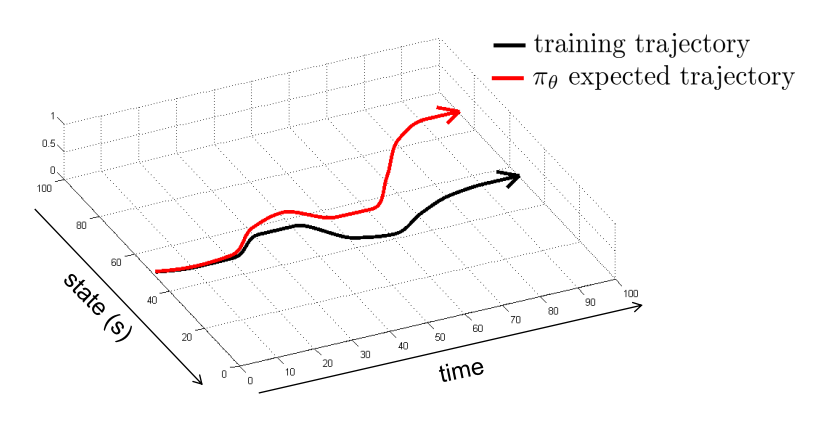
\includegraphics[scale=0.4]{figures/imitation_learning.png}
    %         \end{figure}

    %     \end{frame}

    \section{Reinforcement Learning}

        \begin{frame}
            \frametitle{Markov Decision Process}
            Markov Decision Process is a 4-tuple $(S, A, T, r)$:
            \begin{itemize}
                \item $S$: space of states $s$;
                \item $A$: space of actions $a$;
                \item $T$: transition operator, with probabilities $P(s_{t+1} | s_t, a_t)$;
            \item $r$: reward function $S \times A \rightarrow {\rm I\!R}, \ (s, a) \mapsto r(s, a)$.
            \end{itemize}
        \end{frame}

        \begin{frame}
            \frametitle{The goal of Reinforcement Learning}
            \begin{figure}
                \centering
                \caption{Reinforcement Learning world (\href{http://rail.eecs.berkeley.edu/deeprlcourse-fa18/static/slides/lec-4.pdf}{Deep RL Berkeley Course}).}
                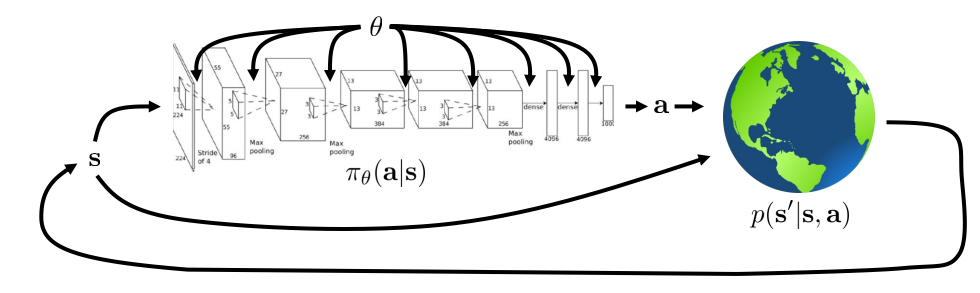
\includegraphics[width=0.9\linewidth]{figures/goal_rl.png}
                \label{fig:1}
            \end{figure}
            $$p_{\theta}(\tau) = p_{\theta}(s_1, a_1, \cdots, s_T, a_T) = p(s_1) \prod_{t=1}^T \pi_{\theta}(a_t|s_t)p(s_{t+1}|s_t, a_t)$$
            $$\theta^* = \arg\max_\theta E_{\tau \sim p_\theta(\tau)}\left[\sum_t r(s_t, a_t)\right]$$
        \end{frame}

        \begin{frame}
            \frametitle{Too many algorithms}
            \begin{itemize}
                \item Policy iteration;
                \item Value iteration;
                \item Q-learning;
                \item Deep Q-learning.
            \end{itemize}
        \end{frame}

        \begin{frame}
            \frametitle{More definitions}
            \begin{block}{Q-Function}
                $$Q^\pi(s_t, a_t) = \sum_{t'=t}^T E_{\pi_\theta}[r(s_{t'}, a_{t'})|s_t, a_t]$$

                The total expected reward for taking an action $a_t$ when the state is $s_t$.
            \end{block}
            \begin{block}{Value Function}
                $$V^\pi(s_t) = E_{a_t \sim \pi_\theta(a_t|s_t)}[Q^\pi(s_t, a_t)]$$

                The total expected reward when the state is $s_t$.
            \end{block}
        \end{frame}

        \begin{frame}
            \frametitle{Policy iteration}
            \begin{figure}
                \centering
                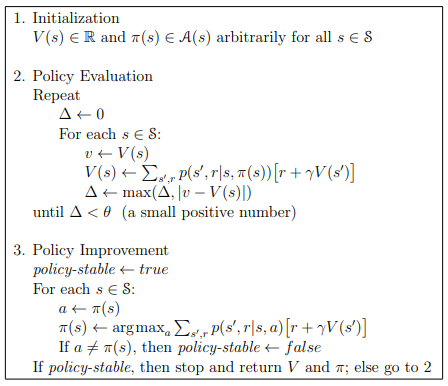
\includegraphics[width=0.6\linewidth]{figures/policy_iteration.png}
                \label{fig2:policy}
                \caption{Policy iteration (Sutton and Andrew, Reinforcement Learning: An Introduction, 2nd edition).}
            \end{figure}
        \end{frame}

        \begin{frame}
            \frametitle{Policy iteration example: FrozenLake8x8}
            \begin{figure}
                \centering
                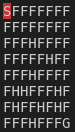
\includegraphics[width=0.2\linewidth]{figures/frozenlake8x8}
                \label{fig4:frozenlake8x8}
                \caption{FronzenLake8x8 environment.}
            \end{figure}
        \end{frame}

        \begin{frame}
            \frametitle{Value iteration}
            \begin{figure}
                \centering
                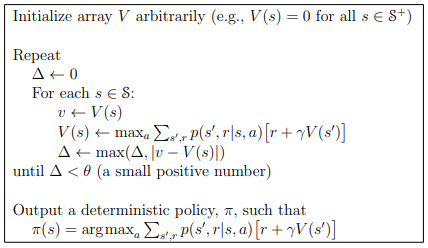
\includegraphics[width=0.7\linewidth]{figures/value_iteration.png}
                \label{fig5:value}
                \caption{Value iteration (Sutton and Andrew, Reinforcement Learning: An Introduction, 2nd edition).}
            \end{figure}
        \end{frame}

        \begin{frame}
            \frametitle{Value iteration example: FrozenLake8x8}
            \begin{figure}
                \centering
                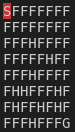
\includegraphics[width=0.2\linewidth]{figures/frozenlake8x8}
                \label{fig6:frozenlake8x8}
                \caption{FronzenLake8x8 environment.}
            \end{figure}
        \end{frame}

        \begin{frame}
            \frametitle{Q-Learning}
            \begin{figure}
                \centering
                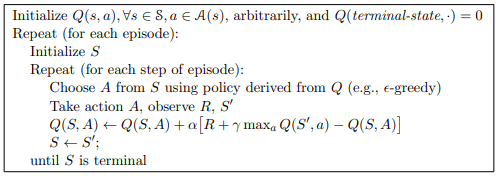
\includegraphics[width=0.8\linewidth]{figures/q_learning.png}
                \label{fig6:q}
                \caption{Q-Learning (Sutton and Andrew, Reinforcement Learning: An Introduction, 2nd edition).}
            \end{figure}
        \end{frame}

        \begin{frame}
            \frametitle{Q-Learning example}
            \begin{figure}
                \centering
                \fbox{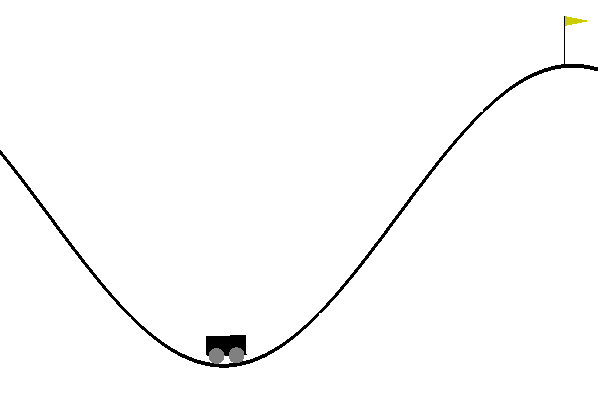
\includegraphics[width=0.7\linewidth]{figures/mountaincar.png}}
                \label{fig7:mountain}
                \caption{MountainCar enviroment.}
            \end{figure}
        \end{frame}

        \begin{frame}
            \frametitle{Approximate Q-Learning}
            We assume the existence of a feature function $f: (s, a) \mapsto f_1(s, a), \cdots, f_n(s, a)$, with $f_i(s, a)$ a feature value.
            \begin{block}{Approximate Q-Function}
                $$Q(s, a) = \sum_{i = 1}^n f_i(s, a) w_i$$
            \end{block}
            \begin{block}{Approximate Q-learning iteration}
                $$w_i \leftarrow w_i + \alpha \cdot difference \cdot f_i(s, a)$$
                $$difference = (r + \gamma \max_{a'} Q(s', a')) - Q(s, a)$$
            \end{block}
        \end{frame}

        \begin{frame}
            \frametitle{Approximate Q-Learning example}
            \begin{figure}
                \centering  
                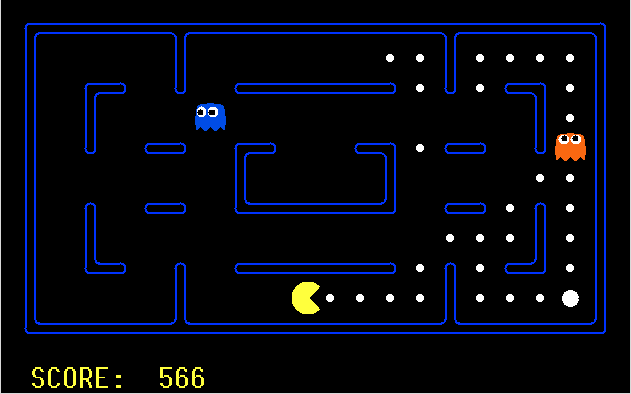
\includegraphics[width=0.8\linewidth]{figures/pacman.png}              
                \caption{PacMan environment (\href{http://ai.berkeley.edu/reinforcement.html}{Berkeley Intro to AI}).}
                \label{fig8:pacman}
            \end{figure}
        \end{frame}

    \section{Deep Reinforcement Learning}

        \begin{frame}
            \frametitle{Deep Q-Learning with Experience Replay}
            \begin{figure}
                \centering
                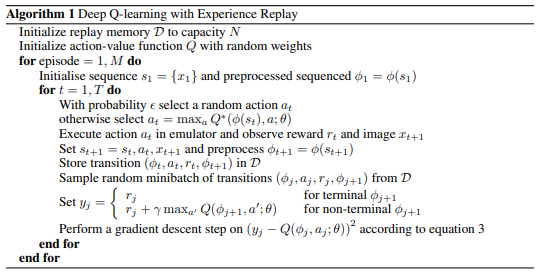
\includegraphics[width=0.8\textwidth]{figures/deep_q_learning}
                \caption{Deep Q-Learning algorithm (\href{https://arxiv.org/pdf/1312.5602v1.pdf}{DeepMind, Playing Atari with Deep Reinforcement Learning}).}
                \label{fig9:deep-q}
            \end{figure}
        \end{frame}

        \begin{frame}
            \frametitle{Deep Q-Learning with Experience Replay example}
        
            \begin{figure}[]
                \begin{figure}
                    \centering
                    \fbox{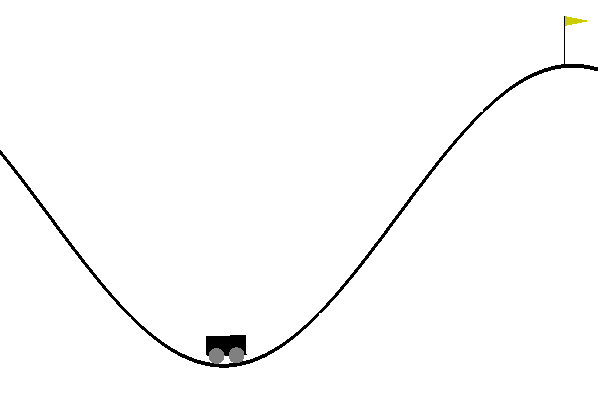
\includegraphics[width=0.7\linewidth]{figures/mountaincar.png}}
                    \label{fig10:mountain2}
                    \caption{MountainCar enviroment.}
                \end{figure}
            \end{figure}
        
        \end{frame}

    \section{What's next}

        \begin{frame}
            \frametitle{Deep Q-Learning + CNN}
        
            \begin{itemize}
                \item Learn from a game image;
                \item Use convolutional neural networks to learn to treat this image.
            \end{itemize}

            \begin{figure}[]
                \centering
                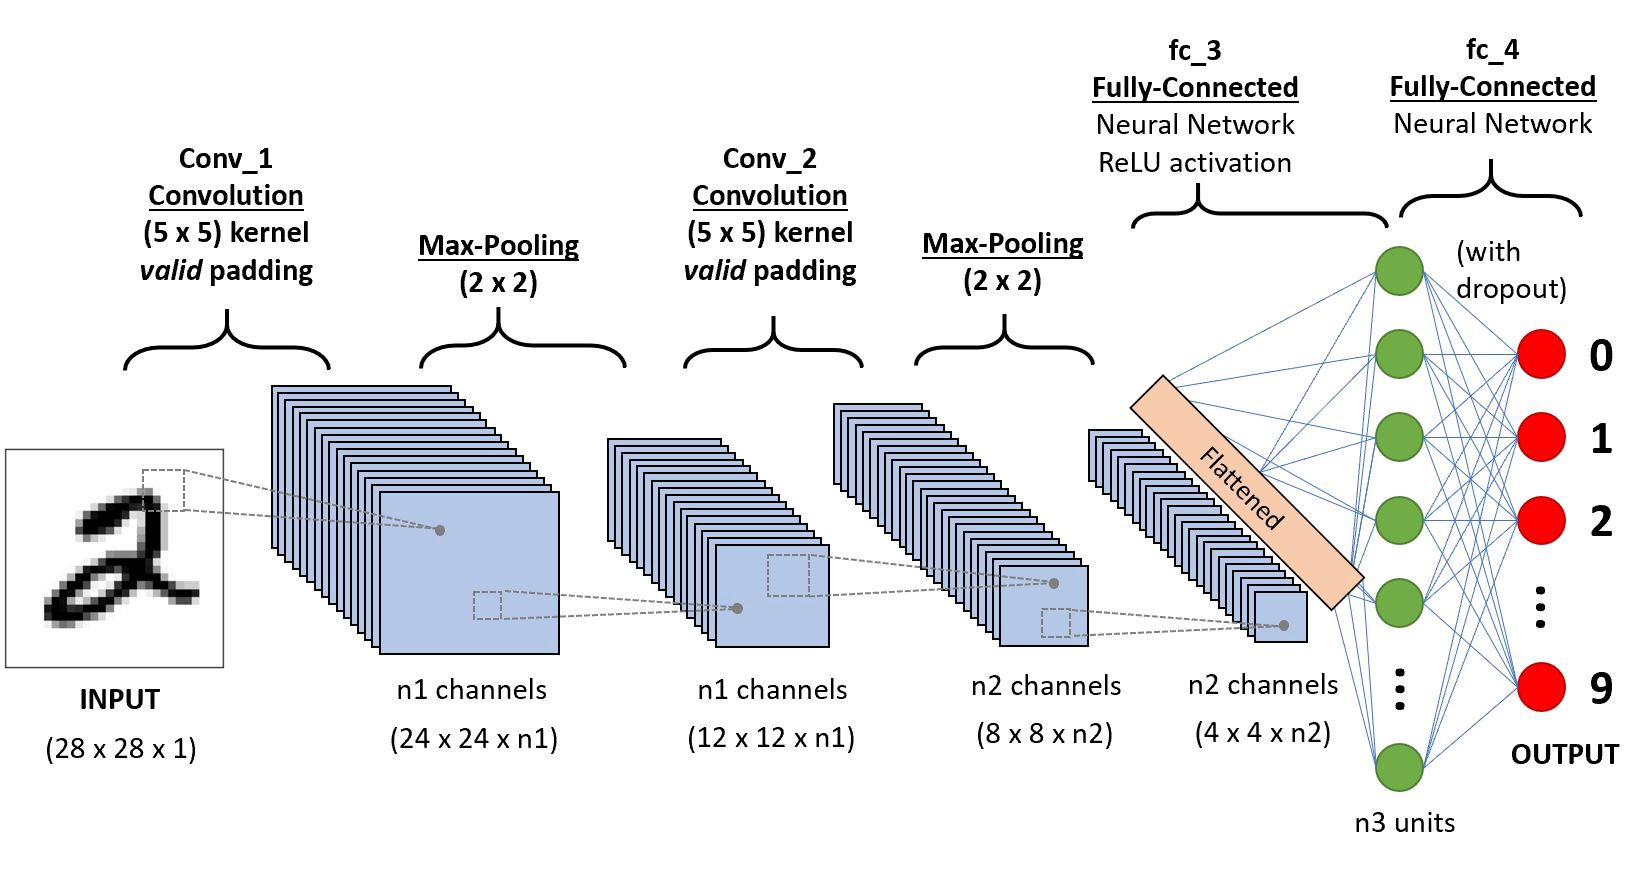
\includegraphics[width=0.7\textwidth]{figures/cnn}
                \caption{Convolutional Neural Network example (\href{https://towardsdatascience.com/a-comprehensive-guide-to-convolutional-neural-networks-the-eli5-way-3bd2b1164a53}{Saha, A Comprehensive Guide to Convolutional Neural Networks — the ELI5 way}).}
                \label{fig11:cnn}
            \end{figure}
        
        \end{frame}

        \begin{frame}
            \frametitle{Atari 2600}
            
            \begin{figure}[]
                \centering
                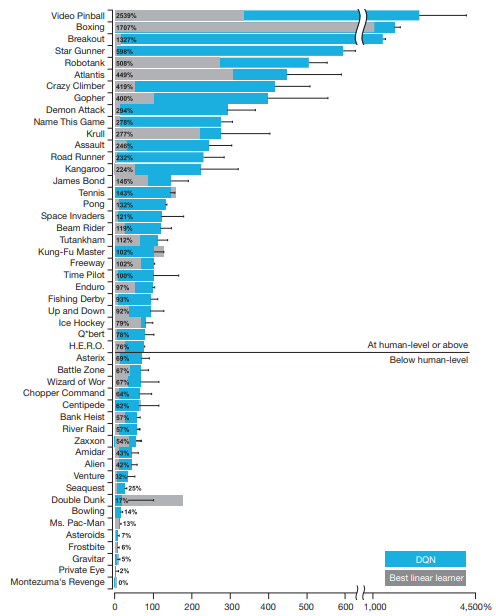
\includegraphics[height=0.7\textheight]{figures/comparison1}
                \caption{Comparison of DQN with linear methods, both normalized by professional players (100\%) and random players (0\%) (\href{https://storage.googleapis.com/deepmind-data/assets/papers/DeepMindNature14236Paper.pdf}{Human-level control through deep reinforcement learning}).}
                \label{fig12:atari}
            \end{figure}
        
        \end{frame}

        \begin{frame}
            \frametitle{Atari 2600}
            
            \begin{figure}[]
                \centering
                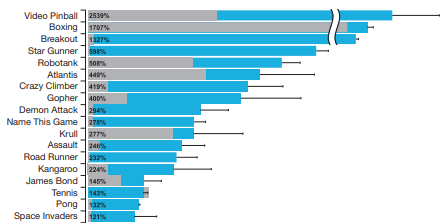
\includegraphics[width=0.8\textwidth]{figures/comparison2}
                \caption{Comparison of DQN with linear methods, both normalized by professional players (100\%) and random players (0\%) (\href{https://storage.googleapis.com/deepmind-data/assets/papers/DeepMindNature14236Paper.pdf}{Human-level control through deep reinforcement learning}).}
                \label{fig12:atari}
            \end{figure}
        
        \end{frame}

        \begin{frame}
            \frametitle{Super Mario Bros.}
        
            \begin{figure}
                \centering
                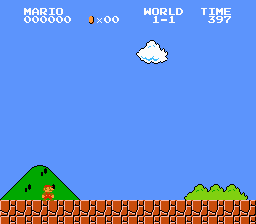
\includegraphics[width=0.6\textwidth]{figures/super_mario_bros.png}
                \caption{Super Mario Bros. Open AI environment (\href{https://pypi.org/project/gym-super-mario-bros/}{PyPI}).}
                \label{fig13:mario}
            \end{figure}
        
        \end{frame}

    \section{Partial considerations}

        \begin{frame}
            \frametitle{Partial considerations}
        
            \begin{itemize}
                \item Reinforcement Learning \& Deep Reinforcement Learning today consist in many algorithms, so that many chalenging problems can be solved with them;
                \item We have today different powerful world applications, and many great things are being done.
                \item There are many paths to follow in order to learn and to research.
            \end{itemize}
        
        \end{frame}

        \begin{frame}
            \frametitle{Thank you}
        
            \epigraph{``Instead of trying to produce a program to simulate the adult mind, why not rather try to produce one which simulates the child's? If this were then subjected to an appropriate course of education one would obtain the adult brain."}{--- \textup{Alan Turing}}
        
        \end{frame}
    
\end{document}